\documentclass[a4paper,11pt]{article}
\input{/home/gilles/Dropbox/preambule_lycee}

\numpage

\begin{document}
\entete{}{R1}{}



\vspace{2.3cm}

\scalebox{0.5}{
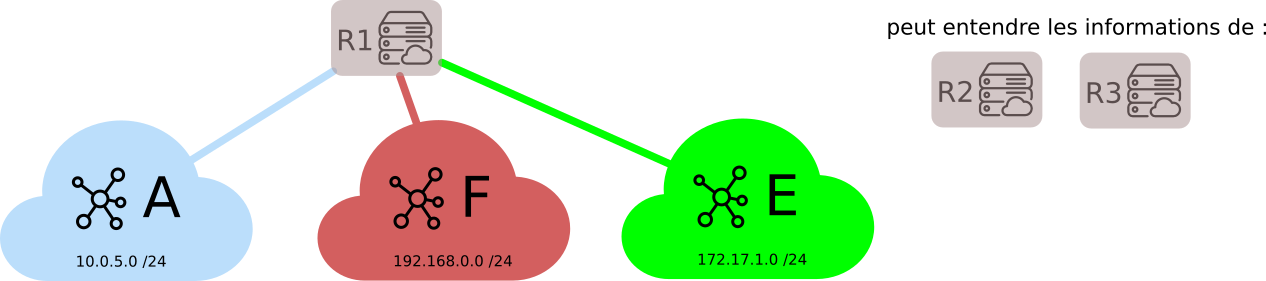
\includegraphics{data/R1.png}
}


\vspace{1.3cm}

\seccg{Tour \no0}


\begin{center}
\renewcommand{\arraystretch}{1.5}
\newcolumntype{M}{>{\centering}m{1cm}}
\begin{tabular}{|c|c|c|}
\hline 
\textbf{Réseau accessible} & \textbf{En passant par}  &	\textbf{Distance}  \tabularnewline
\hline
 &  &  \tabularnewline
\hline
 &  &  \tabularnewline
\hline
 &  &  \tabularnewline
\hline
 &  &  \tabularnewline
\hline
 &  &  \tabularnewline
\hline
 &  &  \tabularnewline
\hline
\end{tabular}

\end{center}


\seccg{Tour \no1}


\begin{center}
\renewcommand{\arraystretch}{1.5}
\newcolumntype{M}{>{\centering}m{1cm}}
\begin{tabular}{|c|c|c|}
\hline 
\textbf{Réseau accessible} & \textbf{En passant par}  &	\textbf{Distance}  \tabularnewline
\hline
 &  &  \tabularnewline
\hline
 &  &  \tabularnewline
\hline
 &  &  \tabularnewline
\hline
 &  &  \tabularnewline
\hline
 &  &  \tabularnewline
\hline
 &  &  \tabularnewline
\hline
\end{tabular}

\end{center}

\seccg{Tour \no2}


\begin{center}
\renewcommand{\arraystretch}{1.5}
\newcolumntype{M}{>{\centering}m{1cm}}
\begin{tabular}{|c|c|c|}
\hline 
\textbf{Réseau accessible} & \textbf{En passant par}  &	\textbf{Distance}  \tabularnewline
\hline
 &  &  \tabularnewline
\hline
 &  &  \tabularnewline
\hline
 &  &  \tabularnewline
\hline
 &  &  \tabularnewline
\hline
 &  &  \tabularnewline
\hline
 &  &  \tabularnewline
\hline
\end{tabular}

\end{center}


\end{document}


